\chapter{Dataset e Machine Learning}


\section{Generazione del dataset}
\label{sec:costruzione-dataset}
Per ottenere un dataset affidabile, è necessario definire i parametri delle simulazioni, stabilendo quali mantenere costanti e quali variare. Questa scelta permette di studiare come le condizioni orbitali influenzino l'evoluzione degli ammassi stellari, mantenendo invariate le altre caratteristiche del sistema.
\subsection{Parametri dell'ammasso stellare}
\label{subsec:condizioni-iniziali}
L'ammasso stellare viene inizializzato secondo il modello di Plummer, descritto nella Sezione~\ref{subsec:plummer}. In tutte le simulazioni vengono fissati il numero di stelle, $\numberOfStars=200$, il parametro di scala $\clusterRadius=1.0$ e la massa totale $\totalMass=1.0$.\\
Le stelle hanno tutte la stessa massa, calcolata come:
\begin{equation}
	\starMass=\frac{\totalMass}{\numberOfStars}=0.005.
	\label{eq:massa-singola-stella}
\end{equation}
Per ottenere diverse realizzazioni iniziali dell'ammasso vengono utilizzati 15 semi di generazione distinti, che determinano differenti distribuzioni iniziali delle posizioni e delle velocità stellari. In questo modo è possibile valutare l'influenza delle condizioni iniziali sui risultati, evitando di basare l'analisi su una singola realizzazione dell'ammasso.
\subsection{Parametri galattici ed orbitali}
\label{subsec:parametri-orbitali}
Il potenziale gravitazionale esterno è descritto dal modello di Plummer, introdotto nella Sezione~\ref{subsec:plummer-galattico}, con massa galattica $\galaxyMass=3000.0$ e parametro di scala $\galaxyRadius=20.0$, mantenuti costanti in tutte le simulazioni.
Le orbite sono definite mediante il semiasse maggiore $\semiMajorAxis$ e l'eccentricità $\orbitEccentricity$. Il primo assume 30 valori compresi tra $10.0$ e $300.0$, con incrementi di $10.0$:
\[
\semiMajorAxis \in \{10,20,30,\ldots,290,300\}.
\]
L'eccentricità assume invece 38 valori compresi tra $0.0$ e $0.925$, con incrementi di $0.025$:
\[
\orbitEccentricity \in \{0,0.025,0.050,\ldots,0.900,0.925\}.
\]
Considerando tutte le combinazioni dei due parametri, si ottengono $30\times38=1140$ configurazioni orbitali. Ciascuna viene utilizzata per diverse realizzazioni iniziali dell'ammasso, così da studiare l'evoluzione del sistema al variare delle dimensioni e della forma dell'orbita.
\subsection{Parametri di integrazione}
\label{subsec:parametri-integrazione}
Le simulazioni adottano una costante gravitazionale $\gravitationalConstant=1.0$, scelta che consente di esprimere tutte le grandezze in un sistema di unità coerente, evitando conversioni tra diverse unità di misura. L'integrazione numerica viene eseguita con il metodo leapfrog \cite{hairer2006geometric}, utilizzando un passo temporale $\deltat=0.005$. Per regolarizzare il potenziale gravitazionale durante gli incontri ravvicinati tra le stelle, viene adottato un parametro di ammorbidimento pari a $\softeningLength=0.01$.
Il tempo finale delle simulazioni è fissato a $\simulationEndTime=700.0$, per contenere l'influenza della dissoluzione dell'ammasso dovuta alla sua evoluzione dinamica interna e concentrarsi sugli effetti della rimozione mareale galattica \cite{cai2016evolution}.
\subsection{Riepilogo dei parametri}
\label{subsec:riepilogo-parametri}
La Tabella~\ref{tab:parametri-dataset} riassume i parametri adottati per le simulazioni, distinguendo quelli mantenuti costanti da quelli variati per esplorare le diverse configurazioni orbitali.
\begin{table}[htbp]
	\centering
	\caption{Parametri adottati per la generazione del dataset.}
	\label{tab:parametri-dataset}
	\begin{tabular}{lll}
		\hline
		\textbf{Parametro} & \textbf{Simbolo} & \textbf{Valore} \\
		\hline
		\multicolumn{3}{l}{\textit{Ammasso stellare}} \\
		Numero di stelle & $\numberOfStars$ & $200$ \\
		Massa totale & $\totalMass$ & $1.0$ \\
		Massa di una stella & $\starMass$ & $0.005$ \\
		Parametro di scala del modello di Plummer & $\clusterRadius$ & $1.0$ \\
		Numero di semi generativi utilizzati & --- & $15$ \\
		\hline
		\multicolumn{3}{l}{\textit{Potenziale galattico}} \\
		Massa galattica & $\galaxyMass$ & $3000.0$ \\
		Parametro di scala galattico & $\galaxyRadius$ & $20.0$ \\
		\hline
		\multicolumn{3}{l}{\textit{Parametri orbitali}} \\
		Semiasse maggiore & $\semiMajorAxis$ & $[10.0,\,300.0]$, passo $10.0$ \\
		Eccentricità & $\orbitEccentricity$ & $[0.0,\,0.925]$, passo $0.025$ \\
		\hline
		\multicolumn{3}{l}{\textit{Integrazione numerica}} \\
		Costante gravitazionale & $\gravitationalConstant$ & $1.0$ \\
		Passo temporale & $\deltat$ & $0.005$ \\
		Parametro di ammorbidimento & $\softeningLength$ & $0.01$ \\
		Tempo finale & $\simulationEndTime$ & $700.0$ \\
		Integratore & --- & Leapfrog \\		
		\hline
	\end{tabular}
\end{table}
\section{Analisi del dataset}
\label{sec:analisi-dataset}
Come descritto nelle Sezioni~\ref{subsec:condizioni-iniziali} e~\ref{subsec:parametri-orbitali}, vengono considerate $15$ realizzazioni iniziali dell'ammasso, ciascuna evoluta per $1140$ configurazioni orbitali, ottenute combinando i $30$ valori del semiasse maggiore con i $38$ valori dell'eccentricità. Il dataset comprende quindi un totale di $15\times1140=17100$ simulazioni.
\subsection{Distribuzione delle grandezze finali}
\label{subsec:distribuzione-grandezze-finali}
Per analizzare i risultati delle simulazioni, vengono considerati gli istogrammi della frazione di massa legata finale $\boundMassFraction$ e del rapporto tra il raggio di metà massa finale e quello iniziale, definito come:
\[
\halfMassRadiusRatio=\frac{r_{1/2}}{r_{1/2,0}}
\]
\begin{figure}[htbp]
	\centering
	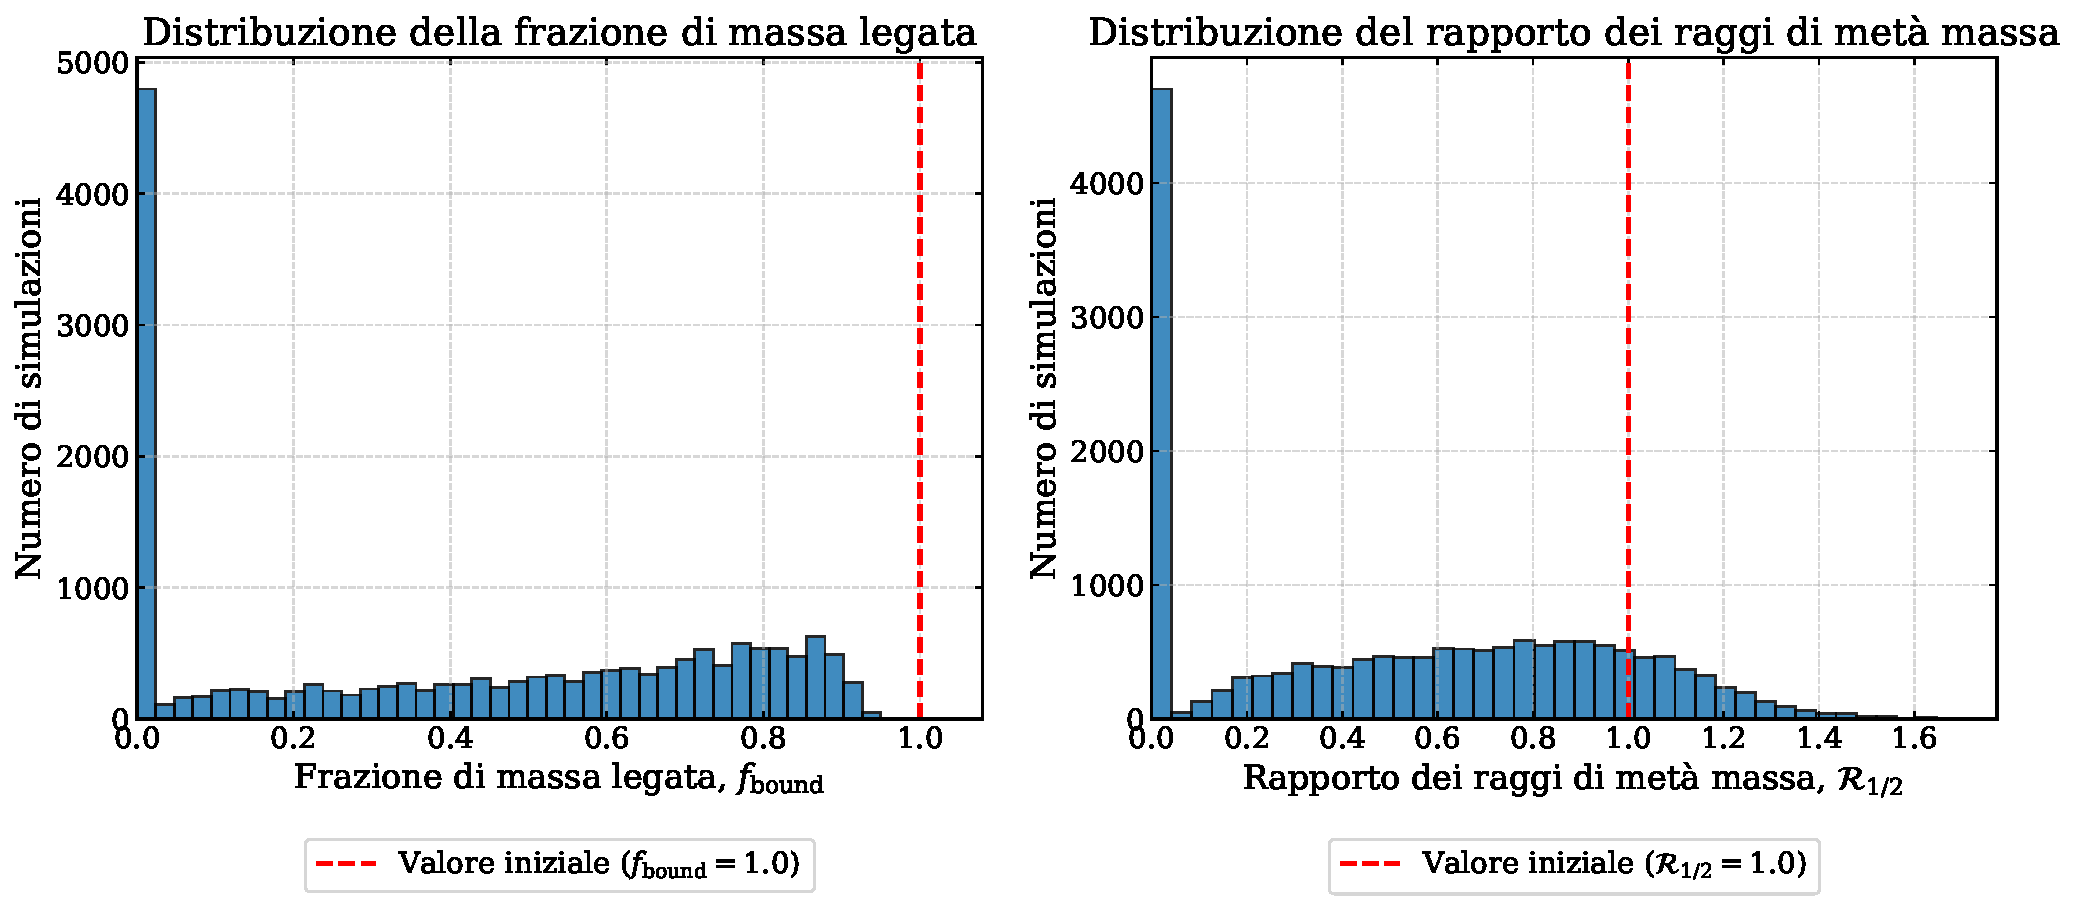
\includegraphics[width=\textwidth]{./plots/distribuzioni_bmf_hmr.pdf}
	\caption{Distribuzione della frazione di massa legata finale $\boundMassFraction$ (a sinistra) e del rapporto tra il raggio di metà massa finale e iniziale $\halfMassRadiusRatio$ (a destra).}
	\label{fig:distribuzione-grandezze-finali}
\end{figure}
Dalla figura~\ref{fig:distribuzione-grandezze-finali} si nota che entrambe le distribuzioni presentano un andamento bimodale, caratterizzato da due gruppi di valori distinti. Si osserva che in $4689$ simulazioni, pari al $27.42\%$ del dataset, sia la frazione di massa legata $\boundMassFraction$ sia il rapporto tra i raggi di metà massa $\halfMassRadiusRatio$ sono nulli. In questi casi, nessuna stella risulta più legata all'ammasso e le stelle si sono totalmente disperse sotto l'effetto delle forze mareali galattiche.
\subsection{Relazione tra parametri orbitali ed esiti delle simulazioni}
\label{subsec:relazione-parametri-esiti}
La Figura~\ref{fig:heatmap-bmf-hmr} mostra le mappe di calore della frazione di massa legata finale $\boundMassFraction$ e del raggio di metà massa finale $R_{1/2}$, in funzione del semiasse maggiore $\semiMajorAxis$ e dell'eccentricità $\orbitEccentricity$. Ogni cella rappresenta la media dei risultati delle $15$ realizzazioni iniziali per una determinata configurazione orbitale.
\begin{figure}[htbp]
	\centering
	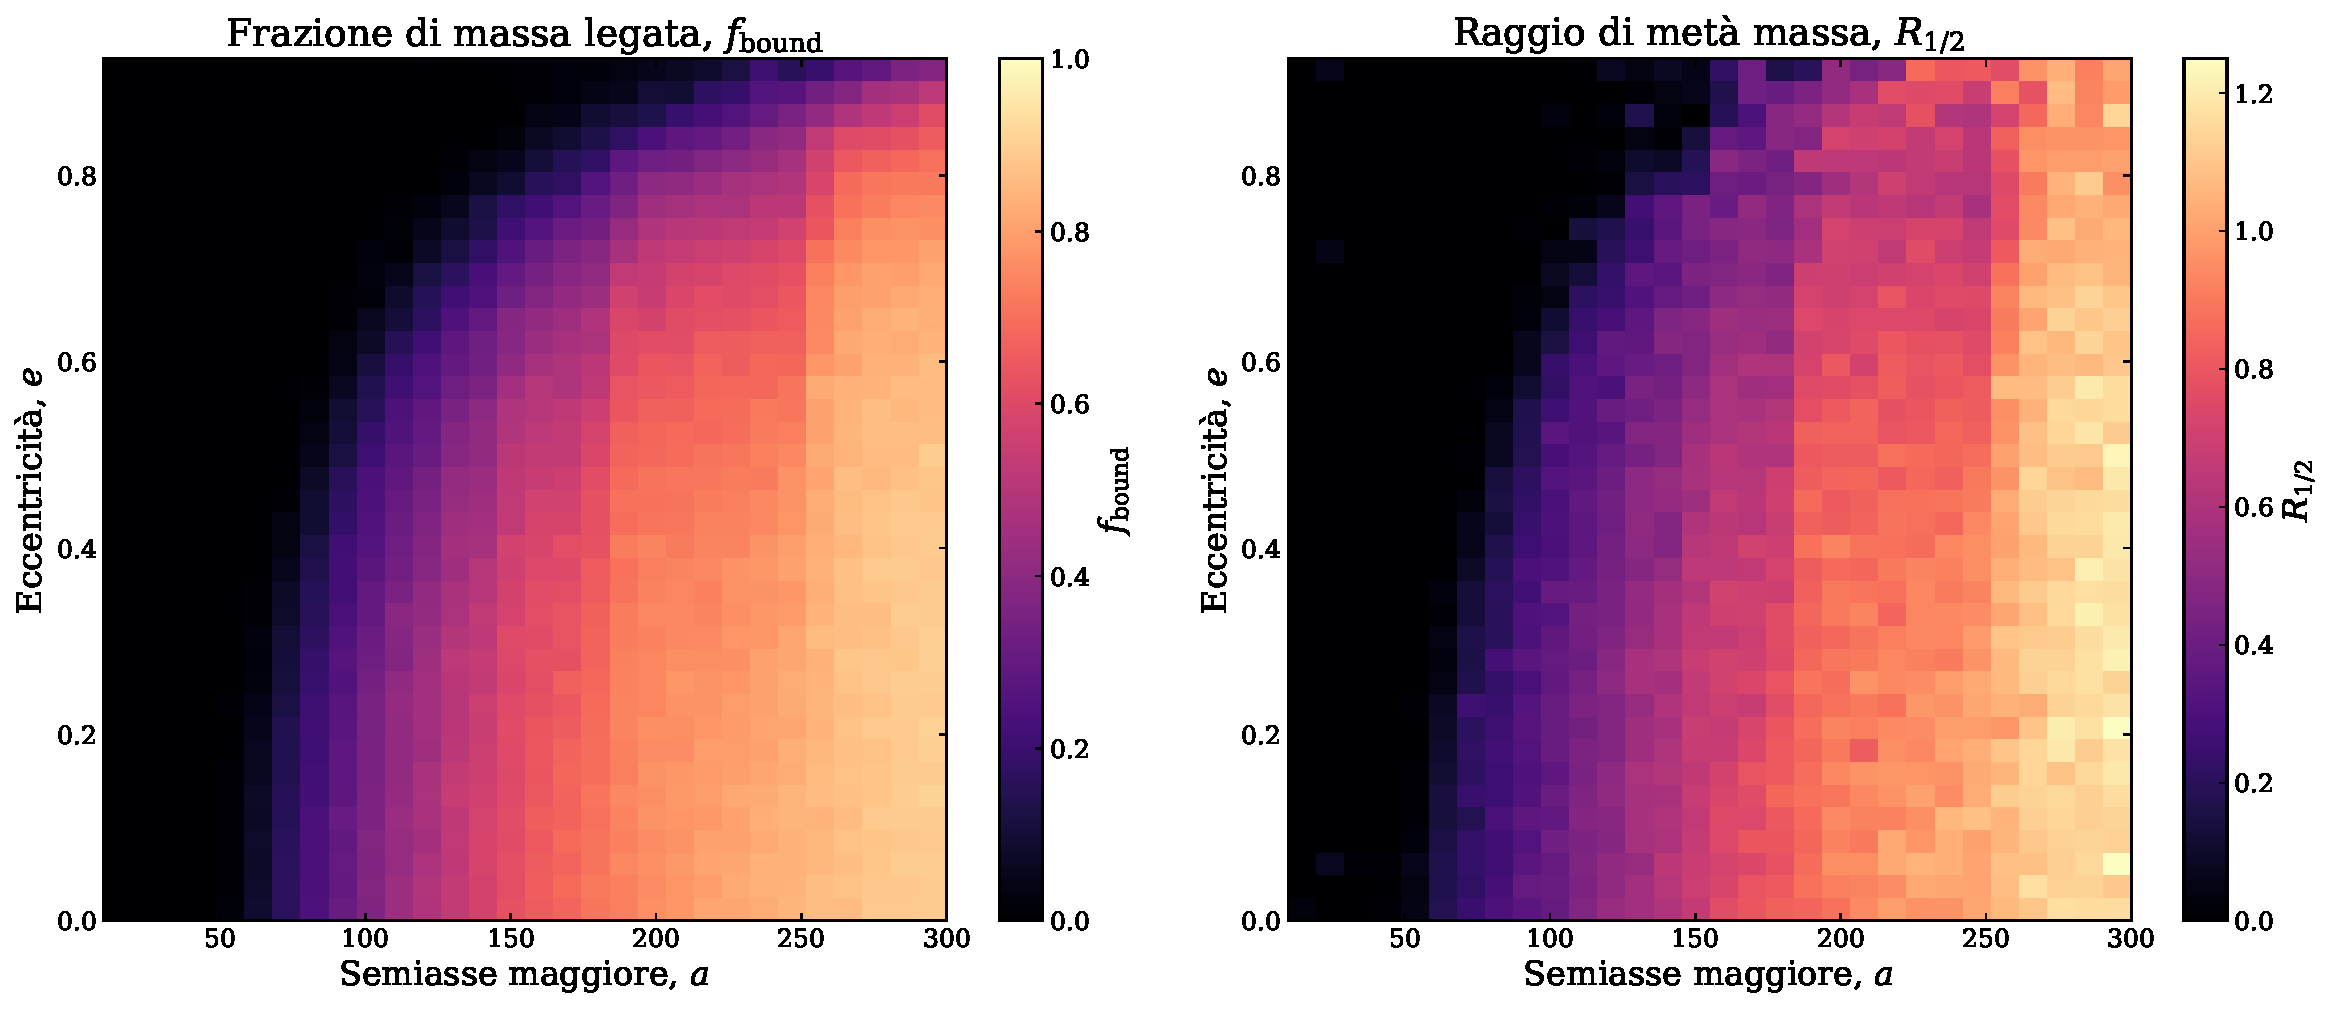
\includegraphics[width=\textwidth]{./plots/mappa_calore_bmf_hmr.pdf}
	\caption{Mappe di calore dei valori medi della frazione di massa legata finale $\boundMassFraction$ (a sinistra) e del raggio di metà massa finale $R_{1/2}$ (a destra), in funzione del semiasse maggiore $\semiMajorAxis$ e dell'eccentricità $\orbitEccentricity$.}
	\label{fig:heatmap-bmf-hmr}
\end{figure}
Le mappe mostrano che per valori del semiasse maggiore inferiori a circa $75$ l'ammasso subisce una dissoluzione completa, dovuta alla forte influenza del potenziale galattico. Anche l'eccentricità influisce sull'evoluzione dell'ammasso: all'aumentare di $\orbitEccentricity$, la dissoluzione diventa progressivamente più marcata, poiché l'ammasso si avvicina maggiormente alla galassia al pericentro, subendo effetti mareali più intensi.


\section{Definizione del problema di classificazione}
\subsection{Classificazione degli ammassi stellari}
\label{subsec:criterio-vivi-morti}
\subsection{Suddivisione in training set e test set}
\label{subsec:suddivisione-dataset}
Per valutare la capacità dei modelli di classificare simulazioni mai viste durante l'addestramento, il dataset viene suddiviso: l'80\% dei dati viene utilizzato per l'addestramento e il restante 20\% per la valutazione finale. La suddivisione è stratificata rispetto alla classe di appartenenza, ovvero viene mantenuta in entrambi gli insiemi la stessa proporzione di ammassi vivi e morti presente nel dataset completo.
\subsection{Standardizzazione delle variabili}
\label{subsec:standardizzazione-variabili}
Il semiasse maggiore e l'eccentricità hanno scale e distribuzioni differenti. Per i modelli sensibili alla scala delle variabili, vengono quindi standardizzati mediante la trasformazione
\[
x' = \frac{x-\mu}{\sigma},
\]
dove $x$ è il valore originale, mentre $\mu$ e $\sigma$ sono rispettivamente la media e la deviazione standard della variabile. Questi parametri vengono calcolati sul training set e utilizzati anche per trasformare il test set, in modo che la valutazione avvenga senza influenzare la fase di addestramento.
\subsection{Albero decisionale}
\label{subsec:albero-decisionale}
\subsection{Support Vector Machine}
\label{subsec:svm}
\subsection{Multi-Layer Perceptron}
\label{subsec:mlp}
\subsection{Regioni decisionali}
\label{subsec:regioni-decisionali}
\subsection{Confronto tramite F1-score}
\label{subsec:confronto-f1-score}